
\section{Introduction}

A target of numerical galaxy evolution studies is to model a representative population of galaxies, resolving all of the relevant physics at the required scales, in order to provide a test bed for the study and interpretation of observed galaxies \citep{benson_galaxy_2010}.
In order to achieve this it is necessary to simulate large volumes (in order to sample a representative volume of the universe) at high resolution (\textit{e.g.} spatial, mass, time; in order to resolve the internal physical processes within individual galaxies) and with all of the key physics included (such as full hydrodynamics, magnetic fields, \textit{etc.}).
Unfortunately this is not computationally feasible; compromises must be made with volume, resolution or choice of physics, depending on the scientific questions posed \citep[for a review, see][]{somerville_physical_2015}.

The most common approach to obtain a representative population of galaxies is to simulate a large periodic cube, tens of Mpc across on a side.
This approach has been used in a number of leading projects to simulate large volumes down to redshift zero, producing thousands of galaxies across a wide range of stellar masses.
Projects such as \eagle\ \citep{schaye_eagle_2015}, Illustris \citep{vogelsberger_introducing_2014}, \textsc{Simba} \citep{dave_simba:_2019} and Horizon-AGN \citep{dubois_dancing_2014} have mass resolutions of order $10^6 \mathrm{M_{\odot}}$, sufficiently high to resolve the internal structure of galaxies.
However, despite these large volumes, the peaks of the overdensity distribution are still poorly sampled due to the lack of large scale modes in constrained periodic volumes.
Much larger volumes are required to sample the rare overdensities on large scales that are likely to evolve in to the most massive clusters by the present day.
For example, the \eagle\ simulation contains just 7, relatively low-mass clusters ($M_{200} > 10^{14} \, \mathrm{M_{\odot}}$) at $z=0$ within the fiducial 100 Mpc volume \citep{schaye_eagle_2015}.

% The Evolution and Assembly of GaLaxies and their Environments (EAGLE) project is a hydrodynamic simulation of galaxy evolution that reproduces many properties of the observed galaxy population at low and intermediate redshifts (\cite{schaye_eagle_2014}, \cite{crain_eagle_2015}).

One means of overcoming the limitations of relatively small periodic volumes is to use much larger, dark matter-only simulations, with box lengths of order Gpc, as sources for \zoom\ simulations.
These use regions selected from the dark matter only simulation as source initial conditions, and resimulate them at higher resolution with extra physics, such as full hydrodynamics \citep{katz_hierarchical_1993, tormen_structure_1997}.
This technique preserves the large scale power by simulating the dark matter at low resolution outside the high resolution region.
A recent example is the \ceagle\ simulations, high resolution, full-hydrodynamic simulations of 30 clusters with a range of descendant masses \citep{barnes_cluster-eagle_2017,bahe_hydrangea_2017}.
These were selected from a parent dark matter simulation with volume $(3.2 \;\mathrm{cGpc})^{3}$ \citep{barnes_redshift_2017}.
This enormous volume contains $185\,150$ clusters ($\mathrm{M_{200}} > 10^{14} \, \mathrm{M_{\odot}}$) and $1701$ high-mass clusters ($\mathrm{M_{200}} > 10^{15} \, \mathrm{M_{\odot}}$).
The \ceagle\ \zoom\ approach allowed the application of the \eagle\ model to cluster environments, without having to simulate a large periodic box.

The zoom technique can also be used to sample a range of overdensities, not just the peaks of the overdensity distribution.
The \textsc{GIMIC} simulations \citep{crain_galaxies-intergalactic_2009} are one example of this approach;
they picked 5 different regions of radius $20$ \cMpch\, at $z = 1.5$ from the Millennium simulation \citep{springel_simulations_2005}, with overdensities (-2,-1,0,1,2)$\sigma$ from the cosmic mean at z = 1.5.\footnote{where $\sigma$ is the \textit{rms} mass fluctuation on the re-simulation scale}
These were then re-simulated at high resolution with full hydrodynamics.
This not only allowed the investigation of the environmental effect of galaxy evolution, without having to simulate a whole periodic box, but also, by appropriately weighting each region according to its overdensity, the regions could be combined to produce composite distribution functions.
These composite functions have much larger dynamic range than those obtained from smaller periodic boxes, and at much lower computational expense than running a large periodic volume.

% In principle, provided a sufficient number of resimulations, this approach could be used to extend the dynamic range of high resolution simulations by sampling the overdense regions and appropriately weighting them with respect to average overdensity resimulations.

In this paper we use a similar approach to GIMIC to produce composite distribution functions of galaxy intrinsic properties, but focused on the Epoch of Reionisation (EoR).
The EoR approximately covers the first 1.2 billion years of the Universe's history ($4 \leqslant z \leqslant 15$), from the birth of the first Population III stars, to when the majority of the intergalactic medium was ionized \citep{bromm_first_2011,zaroubi_epoch_2013,stark_galaxies_2016,cooray_cosmic_2019}.
A number of surveys over the past 15 years, with both space- and ground-based observatories, have discovered thousands of galaxies during this epoch \citep{beckwith_hubble_2006,warren_united_2007,wilkins_new_2011,koekemoer_candels_2011,grogin_candels:_2011,mccracken_ultravista:_2012,bouwens_uv_2015}.
Using intervening clusters as gravitational lenses has pushed the measurement of luminosity functions to even fainter magnitudes \citep{castellano_constraints_2016,livermore_directly_2017,atek_extreme_2018,ishigaki_full-data_2018}.
Spectral energy distribution fitting has been used to characterise the intrinsic properties of these galaxies, measuring for example their stellar masses \citep[\textit{e.g.}][]{gonzalez_evolution_2011,duncan_mass_2014,song_evolution_2016,stefanon_rest-frame_2017} and star formation rates \citep[\textit{e.g.}][]{smit_star_2012,katsianis_evolution_2017}.
However, we have yet to unambiguously detect Population III stars \citep{yoshida_formation_2019}, and the first stages of galaxy assembly are yet to be probed, particularly the seeding and early growth of super massive black holes \citep{smith_first_2017}.

However, this situation may soon change with the introduction of a number of new observatories, each with unique capabilities for exploring the EoR.
\jwst\ will provide unprecedented sensitive imaging with NIRCam, and follow up spectroscopy with NIRSpec and MIRI, to detect and characterise potentially the very first forming galaxies in the Universe \citep{gardner_james_2006}.
In tandem, \wfirst\ and \euclid\ will produce wide-field surveys of the EoR \citep{spergel_wide-field_2015,laureijs_euclid_2011}.
These surveys will predominantly probe the bright end of the rest-frame UV Luminosity Function (UVLF), which is currently poorly constrained by periodic hydrodynamic simulations due to their small volume.
They will also discover some of the most extreme galaxies, in terms of luminosity and intrinsic mass, in the observable universe at these redshifts \citep{behroozi_most_2018}.
These observations will be important to constrain models of galaxy formation and evolution, but it is also possible to predict observed populations in advance and test the recovery of intrinsic parameters \citep{pforr_recovering_2012,pforr_recovering_2013,smith_deriving_2015} Lower et al. 2020, \textit{in prep}.

Predictions for upcoming wide-field surveys have so far typically been made using simple phenomenological models.
One such class of methods are Semi-Analytic Models (SAMs), run on halo merger trees extracted from dark matter-only simulations \citep[for a review, see][]{baugh_primer_2006}.
Due to their simplicity they can be applied to large cosmological volumes, and used to probe distribution functions of intrinsic properties and observables over a large dynamic range.
A number of these models have been tested during the EoR \citep{henriques_galaxy_2015,clay_galaxy_2015,somerville_star_2015, poole_dark-ages_2016, rodrigues_constraints_2017, yung_semi-analytic_2019}.
Mock observables can also be produced and directly compared with observed luminosity functions \citep{lacey_unified_2016,yung_semi-analytic_2019-1,vijayan_detailed_2019}.
Such models can be run relatively quickly, allowing parameter estimation through Monte Carlo approaches \citep{henriques_galaxy_2015}, a powerful means of exploring large degenerate parameter spaces.
However, despite recent progress in resolving SAM galaxies in to multiple components \citep[\textit{e.g.}][]{henriques_l-galaxies_2020}, such models necessarily do not self-consistently model physical processes on small scales, relying on simple recipes.

Most existing periodic hydrodynamic simulations during the EoR are not able to simulate at high resolution the large dynamic ranges accessible by SAMs.
This is illustrated in \fig{volume_resolution}, which shows where a number of existing simulations lie on a plane of simulated volume against hydrodynamic element mass.
There is a strong negative correlation, with some outliers.
The \bluetides\ simulation \citep{feng_bluetides_2016,feng_formation_2015}, based on the Massive Black suite of simulations \citep{matteo_cold_2012,khandai_massiveblack-ii_2015}, was performed within a (500 \,/\,h\,cMpc)$^3$ periodic box, $\sim$125 times as massive as the fiducial \eagle\ volume, whilst at a similar resolution.
They make predictions for a number of intrinsic and observational properties during the EoR \citep[\textit{e.g.}][]{waters_forecasts_2016, di_matteo_origin_2017, wilkins_photometric_2016, wilkins_lyman-continuum_2016, wilkins_properties_2017, wilkins_dust-obscured_2018, wilkins_nebular_2020}
Unfortunately, due to the increased computational cost it has only been run down to $z = 7$, and the model cannot therefore be tested against low redshift observables.
Other simulations have taken a different approach, instead simulating smaller volumes at much higher resolution, allowing them to investigate the effect of a number of physical processes in greater detail \protect\citep{oshea_probing_2015,jaacks_legacy_2019}.
However, these must similarly be stopped at intermediate redshifts due to the higher computational expense.

In this paper we introduce \flares, zoom resimulations during the EoR using the \eagle\ model.
The \eagle\ project \citep{schaye_eagle_2015,crain_galaxies-intergalactic_2009} is a suite of Smoothed Particle Hydrodynamics (SPH) simulations, calibrated to reproduce the stellar mass function and sizes of galaxies in the local universe.
\eagle\ has been shown to be in good agreement with a number of observables not used in the calibration \citep[e.g.][]{lagos_molecular_2015,bahe_distribution_2016,furlong_size_2017,trayford_colours_2015,trayford_optical_2017,crain_eagle_2017}.
This includes predictions at high-$z$: \cite{furlong_evolution_2015} found reasonably good agreement with observationally inferred distribution functions of stellar mass and star formation rate out to $z = 7$.
Unfortunately, there are very few galaxies in the fiducial \eagle\ volume during the EoR.
This is particularly the case for the most massive objects, which predominantly reside in protocluster environments, the progenitors of today's collapsed clusters \citep{chiang_galaxy_2017,lovell_characterising_2018}.
\flares\ allows us to significantly increase the number of galaxies simulated during the EoR with \eagle.
It also allows us to test the already incredibly successful \eagle\ model in a new regime of extreme, high-$z$ environments, whilst still resolving hydrodynamic processes at $10^{6} \, M_{\odot}$ resolution, and provide predictions for a number of key upcoming observatories.

In this, the first \flares\ paper, we introduce the resimulation method, our suite of zoom simulations, and present our first predictions for the distribution of galaxies by stellar mass and star formation rate using the composite approach.
This is the first in a series of papers studying the galaxy properties in the \flares\ sample; in Paper II we forward-model the full spectro-photometric properties, and predict the UV luminosity function and its high redshift evolution (Vijayan et al. 2020, \textit{in prep}).
We assume a Planck year 1 cosmology \citep[$\Omega_{0} = 0.315$, $\Omega_{\Lambda} = 0.685$, $h = 0.673$, ][]{planck_collaboration_planck_2014} and a Chabrier stellar initial mass function (IMF) throughout \citep{chabrier_galactic_2003}.

\begin{figure}
	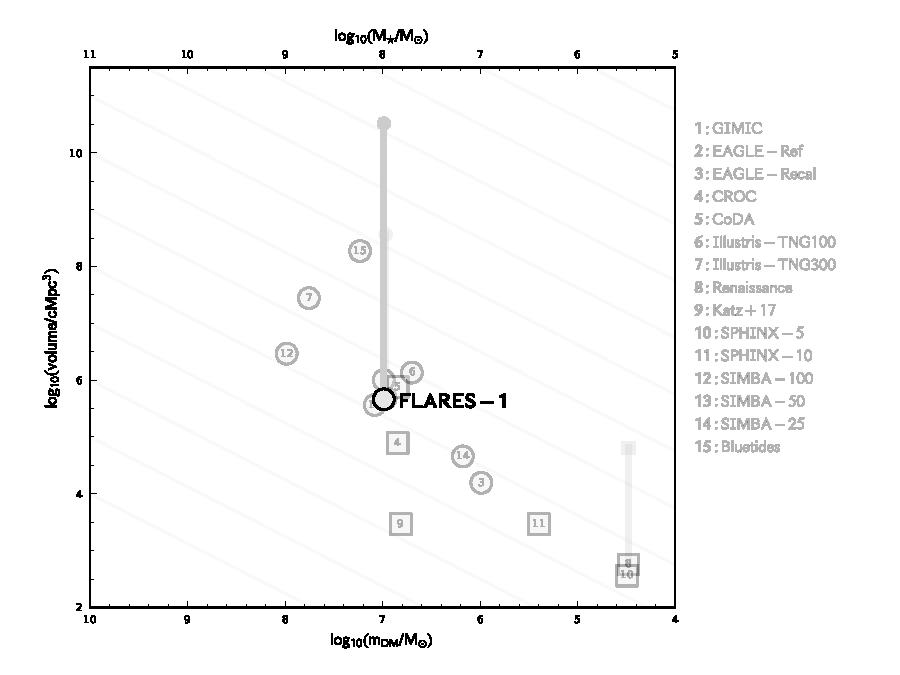
\includegraphics[width=0.5\textwidth]{images/volume_resolution.pdf}
    \caption{Dark matter element resolution against simulated volume.
    We show the following simulation projects: EAGLE \protect\citep{schaye_eagle_2015,crain_eagle_2015}, CROC \protect\citep{gnedin_cosmic_2014}, CoDa \protect\citep{ocvirk_cosmic_2016}, \bluetides\ \protect\citep{feng_bluetides_2016}, Illustris \protect\citep{vogelsberger_introducing_2014}, Renaissance \protect\citep{barrow_first_2017}, SPHINX \protect\citep{rosdahl_sphinx_2018} and the \protect\cite{katz_interpreting_2017} simulations.
    We also show \flares\ with the total re-simulated high-resolution volume and dark matter particle resolution, as well as a vertical line showing the representative volume.
    There is a strong negative correlation for periodic volumes between the volume that can be simulated and the resolution that can be achieved.
    The resimulation approach, with appropriate weighting, allows us to extend the volume axis significantly.
		\todo{update for new figure}
		}
    \label{fig:volume_resolution}
\end{figure}
